% Chapter Template

\chapter{Selection of Compatible Polymer-Solvent Combinations for Near-Field Electrospinning and Pyrolysis} % Main chapter title

\label{Chapter:3}

% search : electrospunable capacity vs. thermo analysis of polymers in solutions (bad/good solvents)

Zhenan Bao et al. \cite{Liu2015a} investigated the effect of the polymer chemical structure (the effect of benzene rings) on the morphology, dimensions, composition, graphitization degree, crystallinity, and electrical conductivity of graphene nano-ribbons derived from four different types of electrospun polymers. The authors studied four polymers polystyrene (PS), poly(vinyl alcohol) (PVA), polyvinylphenol (PVP), and a phenolic resin known as Novolac. See Figure \ref{fig:zhenanBaoPolymers}. The authors created  electrospun polymer fibers out of the four selected polymers. PVP, Novolac and PVA have hydroxyl groups that can be functionalized with metal cations, while PS does not have such binding capability. On the other hand, PVP and Novolac have one benzene ring in each repeating unit, wheras PVA is mainly made out of sp3 carbon.

\begin{figure}[!th]
\centering
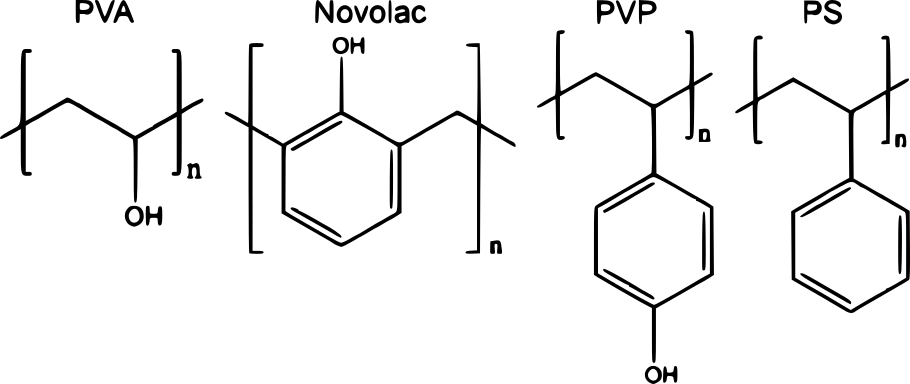
\includegraphics[scale=0.35]{./Figures/zhenanBaoPolymers.png}
\decoRule
\caption[Studied Polymers by Zhenan Bao et al. \cite{Liu2015a}]{Studied Polymers by Zhenan Bao et al. \cite{Liu2015a}}
\label{fig:zhenanBaoPolymers}
\end{figure}

Zhenan Bao et al. \cite{Liu2015a} found that higher sp2 carbon content (or more benzene rings) in the polymer chemical structure translates into higher graphitization degree and higher electrical conductivity in the final carbon structures. This finding can be use as a guide when choosing polymer precursors for the fabrication of carbon structures. Furthermore, the authors posit that polymers with functional groups are required for the creation of smooth and continuous fibers throw electrospinning. \cite{Liu2015a}

%----------------------------------------------------------------------------------------
%	SECTION 1
%----------------------------------------------------------------------------------------
\section{Selection of Candidate Spunable Polymer Solutions}
%high molecular weight, polymer-solution interaction (straight chains)
Given the conclusions from Zhenan Bao et al. \cite{Liu2015a} along with the extensive literature review and data analysis of Chapter \ref{Chapter:2}, the following polymer solutions were selected to be studied in this work. Polymer selection was based on the their high carbon content and presence of benzene rings. The purpose of the polymer selection is to focus the efforts to maximize the likelihood of polymers to yield carbon structures with high electrical conductivity and high graphitization degree; as testing every possible polymer-solvent system is not a practical way to carry on this research. Figure \ref{fig:selectedpolymers} lists the polymers that are going to be investigated. The selected polymers have been electrospun via far-field electrospinning for the fabrication of fibrous mats \cite{Fong1999, Min2013, Yousefi2019}, but no records of being spunable by NFES. 

% 0dot25PEOinSU8_00    % POLY(ETHYLENE OXIDE) in Cyclopentanone
% 21dot21PSinTHF_00    % POLYSTYRENE in TETRAHYDROFURAN
% 15dot0PSBinTHFDMF_00 % POLY(STYRENE-CO-BUTADIENE) in TETRAHYDROFURAN and N,N-DIMETHYLFORMAMIDE
% 15dot0PVKinCHL_00    % POLY(9-VINYLCARBAZOLE) in CHLOROFORM
% XdotXPSMSinDMF       % POLY(STYRENE-CO-ALPHA-METHYLSTYRENE) in N,N-DIMETHYLFORMAMIDE

% 0dot5PVKinSU8_00     % POLY(9-VINYLCARBAZOLE) in Cyclopentanone

% PSB 
% PS  192 000
% PSMS
% PVK 1 100 000
% PEO 4 000 000

\begin{figure}[!th]
\centering
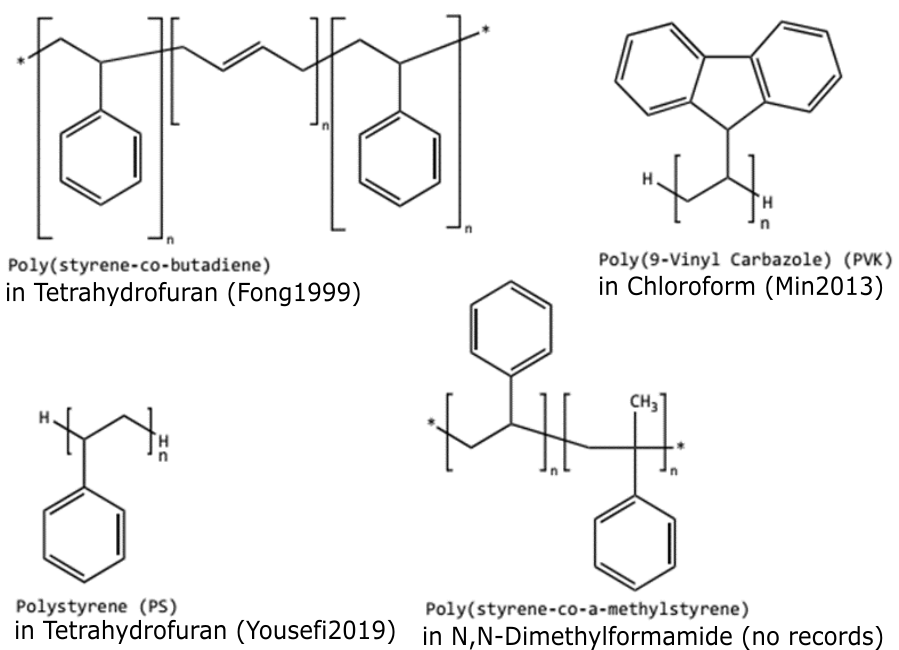
\includegraphics[scale=0.55]{./Figures/selectedpolymers.png}
\decoRule
\caption[Selection of Polymer-Solvent Systems to Investigate in this Work]{Selection of Polymer-Solvent Systems to Investigate in this Work. \cite{Fong1999, Min2013, Yousefi2019}}
\label{fig:selectedpolymers}
\end{figure}

\subsection{Rheology of candidate polymer solutions}
As stated in previous sections, near-field electrospinning requires the control of several parameters to obtain fibers with the desired properties. One of the main parameters are related to the polymer precursor such as molecular weight and its concentration in solution. The evaluation of polymer chain entanglements is an effective way to address the spunability of a polymer-solvent system. \cite{Shenoy2005} Polymer concentration and molecular weight are the main factors in determining the entanglement degree between polymer chains. Solutions at low concentrations do not allow polymer chains to entangle leading the viscoeslasticity od the solution dependent only on individual polymer chains. As the polymer concentration increases, the chains overlap and become entangled. The concentration at which the entanglement initially takes place is the critical concentration $c^*$. Concentrations above the critical concentration $c^*$ generate a fast increase in chain entanglement. This rapid change in chain entanglement is translated into a fast increase in the viscoelasticity of the solution. Figure \ref{fig:concentrationViscosityPlotExplained} illustrates the relationship between polymer concentration and viscoelasticity. \cite{Burghelea2020, Gupta2005}

\begin{figure}[!th]
\centering
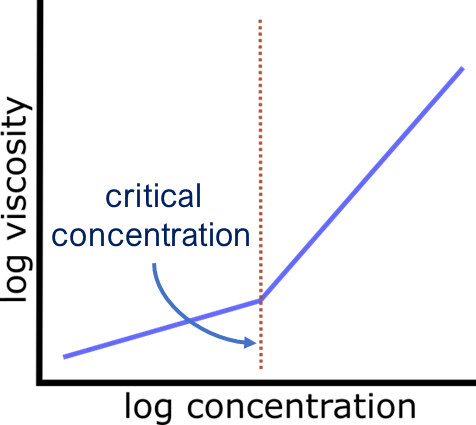
\includegraphics[scale=0.45]{./Figures/concentrationViscosityPlotExplained.png}
\decoRule
\caption[Selection of Polymer-Solvent Systems to Investigate in this Work]{Selection of Polymer-Solvent Systems to Investigate in this Work. \cite{Burghelea2020, Gupta2005, Han2019}}
\label{fig:concentrationViscosityPlotExplained}
\end{figure}

Electrospinning of smooth, continuous fibers require a polymer concentration higher than the critical concentration. As shown in Figure \ref{fig:concentrationViscosityPlotExplained}, the critical concentration can be estimated from the change in slope. \cite{Burghelea2020, Gupta2005, Han2019} 

\subsubsection{Materials and Sample Preparation}
The polymer system studied is SU-8 2002 dissolved in cyclopentanone with poly(ethylene) oxide and tetrabutylammonium tetrafluoroborate as additives, from now on SU-8, PEO and TBATFB. For the experiments, all reactants were used as they arrived. SU-8 was obtained from MicroChem(USA) while PEO and TBATFB 99\% were obtained from Sigma Aldrich (USA). PEO has a viscosity average molecular weight, Mv~4,000,000 with less than 1000 ppm of BHT as inhibitor. For preparing the samples, the adequate amount PEO and TBATFB were added
to 5 mL of SU-8 in a 20mL vial and stirred at 160rpm during 1 hour at 75°C.

The proportions are represented as SU-8:PEO:TBATFB in wt\%. The samples with higher PEO concentration often needed more time of stirring to eliminate all the PEO lumps. In order to avoid any chance of cross-linking of SU-8, during the stirring step, all the samples were isolated from light. To extract the solution from the vial, a syringe of 5mL was used. To eliminate the bubbles from the solution, the syringe was placed upside down during 24 hours before the tests.


%----------------------------------------------------------------------------------------
%	SECTION 1
%----------------------------------------------------------------------------------------
\section{Effect of aromatic groups in oxygen-free polymers in NFES and Pyrolysis}



\section{\emph{conclude with a collection of potential spunable polymer solutions}}